\begin{figure}[h!]
  \centering
    \begin{subfigure}[t]{0.58\linewidth}
    \centering
    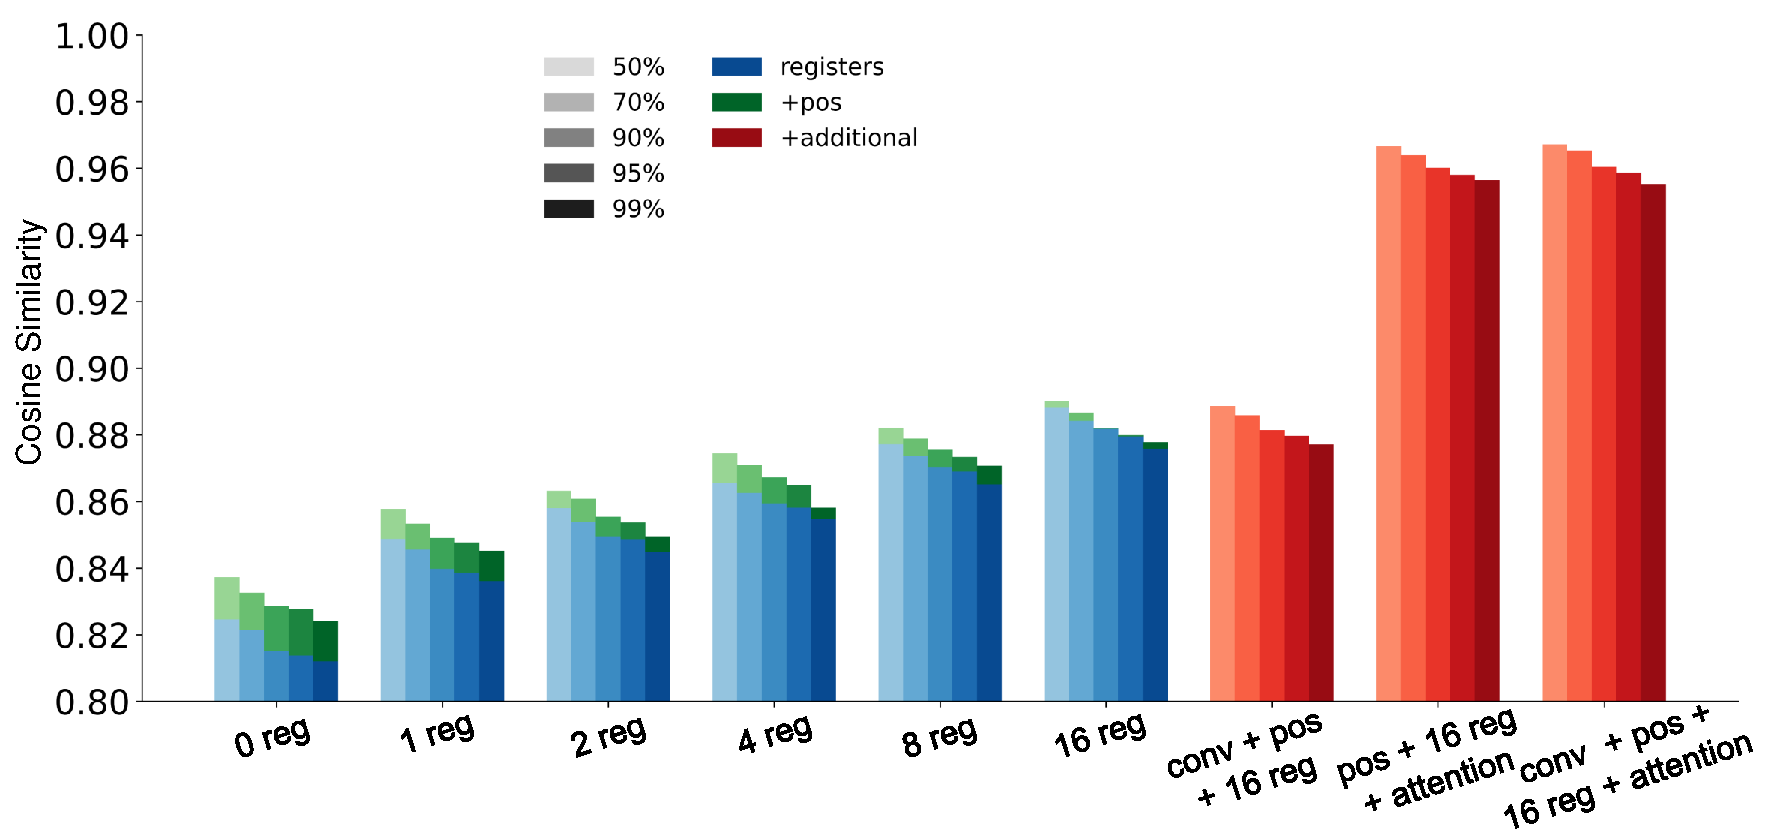
\includegraphics[width=0.98\linewidth]{fig_pdf/ablation_reg_layers_123_cropped.pdf}
    \caption{\textbf{Registers' behavior.} This plot illustrates adding registers improve PH-Reg teacher performance. In the blue settings, only registers are unfreezed. The green settings represent the improvements when positional embeddings are unlocked additionally. The red settings represent performance of unlocking more layers.}
    \label{fig:ablation_reg}
  \end{subfigure}
  \hfill
  \begin{subfigure}[t]{0.38\linewidth}
    \centering
    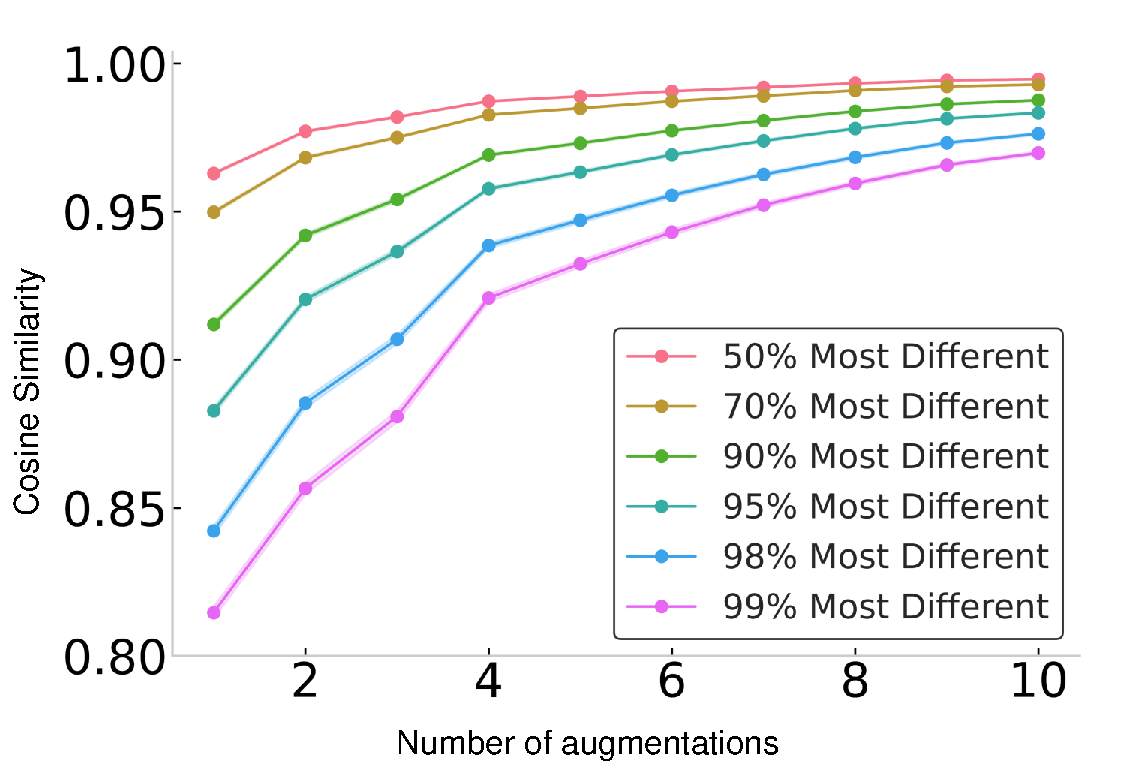
\includegraphics[width=0.98\linewidth]{fig_pdf/num_augmentation.pdf}
    \caption{\textbf{Augmentations improves cosine similarity.} The plot illustrates how increasing the number of augmentations improves the alignment of the model's predictions with the target of 200 augmentations' features, as measured by cosine similarity.}
    \label{fig:ablation_num_of_aug}
  \end{subfigure}
  \hfill
\caption{\textbf{Ablation on number of registers and augmentations} }

\end{figure}